\chapter{Prezentarea Aplicației și Fluxuri}
\label{cap:prezentare}

\section{Fluxul de Autentificare (Login/Logout)}

\begin{enumerate}
  \item User accesează app, redirect la /login (CanActivate guard)
  \item Introduc email și password
  \item Frontend validează client-side (email format, password required)
  \item POST /api/auth/login
  \item Backend verifică credentials, generează JWT token
  \item Frontend salvează token în localStorage
  \item JwtInterceptor adaugă Authorization header
  \item Redirect la /dashboard
  \item Logout: șterge token, redirect /login
\end{enumerate}

\begin{figure}[H]
  \centering
  % \includegraphics[width=0.9\textwidth]{6_SEQUENCE_LOGIN.drawio.png}
  \caption{Sequence Diagram – Fluxul de Autentificare}
  \label{fig:login}
\end{figure}

\section{Dashboard și Navigare Principală}

Dashboard afișează: statistici (total studenți, cursuri, prezență), quick actions, recent activity, sidebar navigation.

\textbf{[Placeholder: screenshot-uri dashboard]}

\section{Modul Studenți (Listare, CRUD, Filtre)}

\subsection{Listare}

Tabel: ID, Name, Email, Group, Year, Status. Paginare, search, sort, filter, action buttons (Edit, Delete).

\subsection{CRUD}

\begin{itemize}
  \item CREATE: Reactive form cu validare (email unique async, name min 3 chars)
  \item READ: Detalii student (cursuri, prezență)
  \item UPDATE: Editare date (email read-only post-creation)
  \item DELETE: Confirmare, refresh lista
\end{itemize}

\textbf{[Placeholder: 4-5 screenshot-uri CRUD]}

\section{Import Excel Studenți (Flux Complet)}

\subsection{Overview}

\begin{figure}[H]
  \centering
  % \includegraphics[width=0.75\textwidth]{11_IMPORT_MINI_OVERVIEW.drawio.png}
  \caption{Import Overview – 4 Pași}
  \label{fig:import-overview}
\end{figure}

\subsection{Validație}

\begin{figure}[H]
  \centering
  % \includegraphics[width=0.8\textwidth]{12_IMPORT_MINI_VALIDATION.drawio.png}
  \caption{Import Validation Decision Tree}
  \label{fig:import-valid}
\end{figure}

\subsection{UI Flow}

\begin{figure}[H]
  \centering
  % \includegraphics[width=0.85\textwidth]{13_IMPORT_MINI_UI_FLOW.drawio.png}
  \caption{Import UX Flow – Upload → Preview → Result}
  \label{fig:import-ux}
\end{figure}

\subsection{Detaliu Proces}

Admin selectează .xlsx file → Frontend validează → POST /api/students/import → Backend parsează cu PHPSpreadsheet → Validează rânduri (email format, group exists, year 1-4) → Insert DB sau erori → Return report JSON → Frontend afișează toast + refresh list.

\begin{figure}[H]
  \centering
  % \includegraphics[width=0.9\textwidth]{5_IMPORT_EXCEL_DATAFLOW.drawio.png}
  \caption{Import Excel Data Flow – Detaliu Complet}
  \label{fig:import-flow}
\end{figure}

\textbf{[Placeholder: 6-8 screenshot-uri import process]}

\section{Modul Prezență (Selectare Sesiune, Marcare, Salvare)}

\begin{enumerate}
  \item Profesor selectează sesiune din dropdown
  \item Frontend fetch-ează lista studenți
  \item Afișare tabel: ID, Name, checkbox (Present/Absent)
  \item Profesor bifează absent pe cei care lipsesc
  \item Click "Submit Attendance"
  \item Frontend validează toți studenții au status
  \item POST /api/attendance/mark
  \item Backend salvează în DB
  \item Toast success + refresh
\end{enumerate}

\begin{figure}[H]
  \centering
  % \includegraphics[width=0.9\textwidth]{7_SEQUENCE_ATTENDANCE_COMPLETE.drawio.png}
  \caption{Sequence Diagram – Marcare Prezență}
  \label{fig:attendance}
\end{figure}

\textbf{[Placeholder: 5-6 screenshot-uri attendance marking]}

\section{Modul Cursuri și Laboratoare}

Tabel cursuri (professor, year, semester) → Click detalii → Laboratoare (1-14 per curs) → Add/Edit/Delete lab.

\textbf{[Placeholder: 2-3 screenshot-uri]}

\section{Modul Examene și Rapoarte}

Upload exam schedule, afișare planning. Rapoarte prezență cu charts, export CSV/PDF, filters.

\textbf{[Placeholder: 2-3 screenshot-uri]}

\section{Administrare (Profesori, Grupe, Permisiuni)}

Admin panel (CanActivate guard): CRUD profesori, grupe, manage permissions, view logs.

\textbf{[Placeholder: 2-3 screenshot-uri]}

\section{Rezultate Vizuale}

\textbf{[Placeholder: Multi-page screenshot gallery]}

\begin{figure}[H]
  \centering
  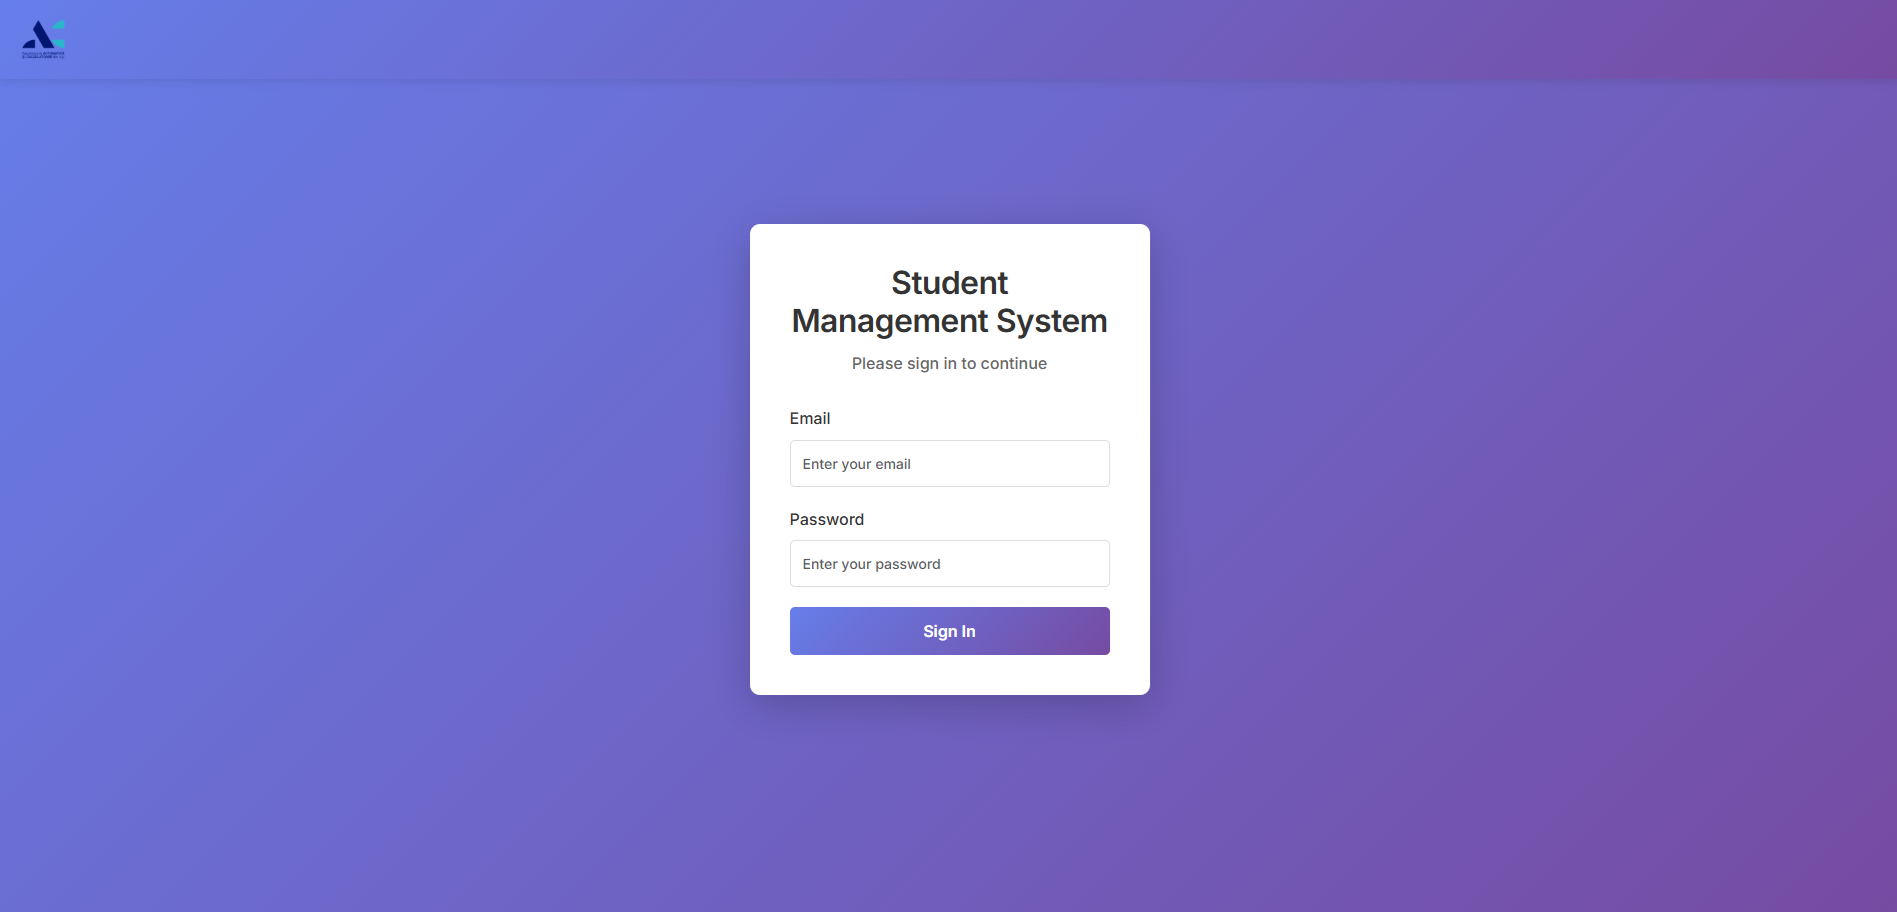
\includegraphics[width=0.95\textwidth]{images/login-page.png}
  \caption{Screenshot – Login Page}
  \label{fig:ss-login}
\end{figure}